\chapter{Обзор предметной области}
\label{cha:analysis}
\section{Цель и задачи работы}
Целью данной работы является создание программного комплекста для обнаружения выбросов временных рядов в собираемых данных.
Для достижения данной цели необходимо решить следующие задачи:
\begin{itemize}
	\item пронализировать предметную область и существующие методы обнаружения выбросов
	\item разработать метод обнаружения выбросов
	\item создать ПО, собирающее данные для анализа
	\item создать ПО, реализующего  разработанный метод обнаружения выбросов
	\item провести вычислительный эксперимент с использованием разработанного метода
	
\end{itemize}
\section{Что такое аномалия}
В анализе данных есть два основных направления, которые занимаются поиском аномалий - это детектирование новизны и обнаружение выбросов. "Объект новизны"\ - это так же объект, который отличается по своим свойствам от объектов  выборки. Однако, в отличие от выброса,  его ещё нет в самой выборке и задача анализа сводится к его обнаружению при появление. Например, если анализировать замеры уровня шума и отбрасывать слишком высокие или слишком низкие значения, то это называется борьбой с выбросами. А если  создаётcя алгоритм, который для каждого нового замера оценивает, насколько он похож на прошлые, и выбрасывает аномальные, то это  назвается "борьбой с новизной"\ .
\cite{Book01}.
Выбросы являются следствием:
\begin{enumerate}
	\item ошибок в данных
	\item неверно классифицированных объектов
	\item присутсвием объектов других выборок
	\item намеренным искажением данных
\end{enumerate}
На рисунке \ref{fig01} находится три вида точек: зеленые, желтые, красные. Множество зеленых точек представляют собой "нормальные" данные. Множество желтых точек означает  выбросы в "слабом смысле". Они незначительно отклоняются от основных  нормальных данных. Красные же точки являются аномальными - выбросами "в сильном смысле"\ . Они значительно  отклоняются  от нормальных данных. В данной работе будет изучаться вопрос находждения "сильных выбросов"\  и  критериев отличия сильного выброса от основных данных. В дальнейшем под словом "выброс"\ будет подразумеваться "сильный выброс"\ ,  а под  аномалией -  выброс(выброс - частный случай аномалии).
Понятие аномалии  интерпетируют по-разному в зависимости от характера данных. Обычно аномалией назыют некоторое отклонение от нормы. В дальнейшем будет дано несколько более формальных опредений аномалий, специфичных для метода их определений.

\section{Обнаружение аномалий}
В машинном обучении обнаружение  "ненормальных" экземпляров в наборах данных всегда представляло большой интерес. Вероятно, первое определение было дано Граббсом\cite{Book02} в 1969 году: "Относительное наблюдение или выброс - это элемент выборки, который, заметно отличается от других членов выборки, в которых он встречается ".
Это определение является актуальным и сегодня, но мотивация для обнаружения аномалий изменилась. Тогда основная причина поиска аномалий заключалась в том, чтобы удалить выбросы из набора данных для обучения, поскольку   используемые алгоритмы, были весьма чувствительны к выбросам в данных. Эта процедура также называется очищением данных. После разработки классификаторов устойчивых к наличию аномалий в обучающем наборе данных, интерес к их поиску угас. Однако, в начале 21 века в связи с развитием интернета и значительным увеличением объема собираемых данных для анализа, исследователи стали больше интересоваться  аномалиями, поскольку они  оказывались часто связаны с особенно интересными событиями.  В этом контексте определение Граббса также было расширено, так что сегодня аномалии имеют две важные характеристики:
\begin{enumerate}
	\item Аномалия отличается от нормы по своим особенностям
	\item Аномалия редко встречается в наборе данных по сравнению с "нормальными"\  данными
\end{enumerate}
\subsection{Классификация методов обнаружений аномалий}
Классическая система классификации предполагает предварительное обучение на обучающем наборе данных и последующую классификацию на основе этого набора. Данные делятся на "обучающую выборку"\ - данные, при помощи которых алогритм обучает классификар и, "тестовую выборку"\ - данные, при анилизе которых, классификатор остается неизменным.Тестовая выборка нужна для того чтобы проверить корректность обучения классификатора.

 Однако, в случае с поиском аномалий, возможны варианты, отличающиеся от классического. Подходящий метод классификации выбирается на основе наличия разметки данных.   Выделяются три основых класса методов:
\begin{enumerate}
\item Обучение с учителем. Для обучения необходимо наличие полностью  размеченных данные для обучения и для тестов. Классификатор  обучается один раз и применяться впоследствии.В связи с тем, что для многих наборов данных заранее неизвестно что является аномалией, а что нет, применение этого метода ограничено.
\item Обучение с частичным привлечением учителя. Для обучения необходимо наличие тествого и учебного набора данных. Однако, в отличие от обучения с привелечением учителя, разметка данных не требуется. Все данные, представленные в выборках, считаются нормальными. На основе этих данных строится некая модель. Все данные, отклоняющиеся от этой модели, считаются аномальными. Эта идея также известна как "одноклассовая" классификация \cite{Book03}.
\item Обучение без учителя.
Самый гибкий способ, который не требует разметки набора данных.  Идея заключается в том, что алгоритм обнаружения аномалий оценивает данные исключительно на основе внутренних свойств набора данных что является нормальным, а что является выбросом. В этой работе основное внимание будет этому  именно этому способу. Так же этот способ называют "неконтролируемый способ обнаружения  аномалий".
\end{enumerate}

\section{Результат метода обнаружения аномалий}
В результате работы алгоритма обнаружения аномалий  с элементом данных связаывается  метка или оценка достоверности(показатель аномальности).  Метка- показатель, который принимает нулевое значения, в случае если она связана с нормальными данными и единицу в противном случае. Оценка показывает вероятность того, что элемент является аномалией. Для разных алгоритмов используется разные шкалы оценок, поэтому приведение конкретных примеров оценок будет некорректным.  В алгоритмах метода обучения с учителем зачастую используются метки как выходные данные, в  алгоритмах  с частичным привлечением учителя и без учителя  обнаружения аномалий чаще встречаются оценки.
\section{Виды аномалий}
\begin{figure}
	\centering
	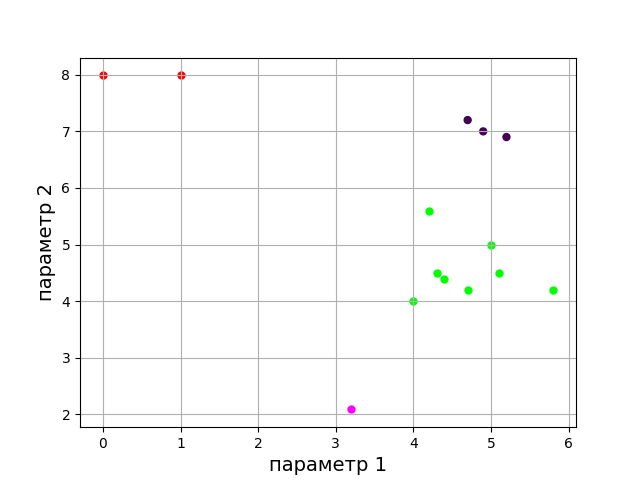
\includegraphics[width=.5\textwidth]{img/1.png}
	\caption{Простой двумерный пример}
	\label{fig01}
\end{figure}

Основная идея алгоритмов обнаружения аномалий заключается в обнаружении экземпляров данных в наборе данных, которые отклоняются от нормы. Однако на практике существует множество случаев, когда это основное предположение является неоднозначным. На рис \ref{fig01} показаны некоторые из этих случаев с использованием простого двумерного набора данных. Две аномалии могут быть легко идентифицированы визуально: красные точки  сильно отличаются отличаются значениям параметров от областей плотной группировки точек. Если смотреть на весь набор данных в целом, то фиолетовую точку можно отнести к тому же классу, что и зеленые точки.  Однако, если сфокусироваься только на кластере зеленых точек и сравнивать его с фиолетовой точкой, пренебрегая всеми другими точками, то её можно рассматривать как аномалию. Поэтому фиолетовая точка называется локальной аномалией, так как она аномальна по сравнению с ее близкой окрестностью. В зависимости от цели анализа, локальные  аномалии могут представлять интерес или нет. 
Другой  вопрос  заключается в том,что следует ли рассматривать точки черного кластера  как три аномалии или как (небольшой) кластер. Такие небольшие кластеры явления называются микрокластерами. Показатели аномальности у точек этого кластера выше, чем  у точек зеленого кластера, но меньше, чем  у красных точек. Этот простой пример  показывает, что задача нахождения аномалий аномалии не всегда тривиальна, а вычисление показателя аномалности иногда полезнее, чем проставление двоичной метки.


Задача обнаружения одиночных аномальных экземпляров  крупном наборе данных называется обнаружением точечных аномалии\cite{Book04}. Сегодня почти все  неконтролируемые алгоритмы обнаружения  относятся к этому типу. Если же аномалии составляют заметный процент, от набора данных, то задачу поиска аномалий называют задачей обнаружения коллектнивных аномалий. Пусть аномалии представляют собой некое множество, тогда необязательно каждый элемент этого множества должен быть аномальным. Возможен вариант когда только определенная их комбинация определяет аномалию.  Третий вид  -  контекстуальные аномалии. Элемент выборке в отрыве от своего контекста может казаться нормальным. Однако, если рассмотреть контекст этого элемента, то очевидным станет его аномальная природа.
 Распространенным контекстом является время. В качестве примера предположим, что  измеряется температура в диапазоне от $-30^{\circ}$C до $+40^{\circ}$C в течение года. Таким образом, температура $25^{\circ}$C кажется довольно нормальной, но когда  учитывается контекстное время (например, месяц), такая высокая температура $25^{\circ}$C  в течение зимы  будет рассматриваться как аномалия.

Алгоритмы обнаружения точечных аномалий так же можно использовать для обнаружения контекстуальных и коллективных аномалий. Для этого нужно включить контекст в алгоритм как параметр алгоритма. В вышеприведенным примере включение месяца как дополнительного параметра поможет обнаружить аномалию. Однако в более сложных сценариях может потребоваться один или несколько новых парметров, чтобы преобразовать задачу определения контекстной аномалии в задачу обнаружения точечной аномалии.  Для того, чтобы преобразовать задачу поиска коллективной аномалии в задачу поиска одиночной, нужно произвести измненения изначального набора данных. Для этого можно использовать корреляцию, агрегация и группировка. Преобразование  может быть нетривиальным.\cite{Book05} . 
Преобразование требует глубоких знаний о наборе исходных данных и часто приводит  к существенным искажениям при переводе данных в новый формат. Такое семантическое преобразование называется  генерированием представления данных(\textit{англ. data view generation}).
  
  Таким образом можно сделать вывод, что многие задачи обнаружения аномалий требуют предварительной обработки данных перед передачей их на вход алгоритму. В противном случае можно получить формально верные, но фактические бесполезные результаты.


Существует большое число алгоритмов для нахождения аномалий. Некоторые из них опирается на априорные данные, некоторые не опираются. Для выбора подходящего алгоритма нахождения аномалий зачастую стоит учитывать характер данных, их размер и доступную априорую информацию. Несмотря на то, область знаний обнаружения аномалий активно развивается как часть современной науки, остается ещё много простора для исследования алгоритмов, модификации и создания новых.
% Обратите внимание, что включается не ../dia/..., а inc/dia/...
% В Makefile есть соответствующее правило для inc/dia/*.pdf, которое
% берет исходные файлы из ../dia в этом случае.

%\begin{figure}
%  \centering
%  \includegraphics[width=\textwidth]{inc/dia/rpz-idef0}
%  \caption{Рисунок}
%  \label{fig:fig01}
%\end{figure}

%\begin{figure}
%  \centering
%  \includegraphics[height=0.85\textheight]{inc/img/leonardo}
%  \caption{Предполагаемый автопортрет Леонардо да Винчи}
 % \label{fig:leonardo}
%\end{figure}

%В \cite{Pup09} указано, что...

